%%
%%  Department of Electrical, Electronic and Computer Engineering.
%%  EPR400/2 Final Report - Technical Documentation.
%%  Copyright (C) 2011-2021 University of Pretoria.
%%

\section{HARDWARE part of the project}

\subsection{Record 1. System block diagram}
\begin{figure}[H]
  \centering
  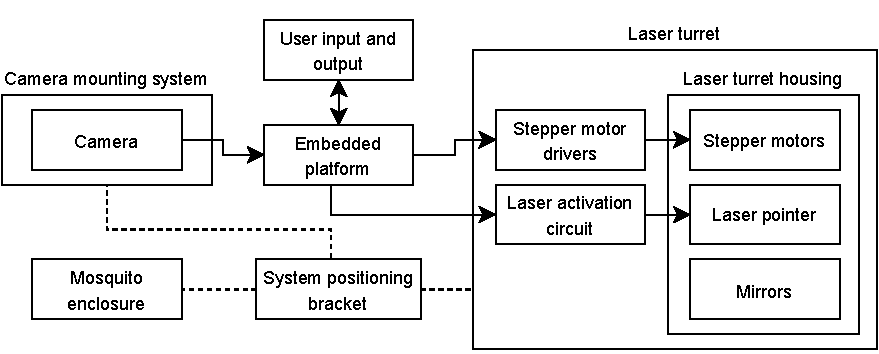
\includegraphics[width=\textwidth]{figures/hardware_block_diagram.pdf}
  \caption{System block diagram.}
\end{figure}

\newpage
\subsection{Record 2.  Systems level description of the design}
The processing for the entire system is done on the Nvidia Jetson Nano. The Jetson Nano reads a frame from the camera. The frame is then processed to detect the position of the mosquitoes and laser reflections. The system updates the mosquitoes tracks. The laser turret target position and the belief position of the laser turret is then updated. The system determines the control action required by the laser turret. The Jetson Nano sends the control signals to the stepper motor drivers. The Jetson Nano is connected to a display, keyboard, and mouse for user interaction. The laser pointer can be powered on and off by the user. The appropriate control signal is sent to the laser activation circuit by the Jetson Nano. The camera, laser pointer, and mosquito enclosure are kept in known positions relative to each other by the system position bracket.

\newpage
\subsection{Record 3. Complete circuit diagrams and description}
A switching transistor circuit was designed to enable the laser to be turned on and off from the Nvidia Jetson Nano \gls{gpio}. The schematic for the switching transistor circuit can be seen in \autoref{fig:transistor_schematic}.  When the input signal is high the transistor is switched on and the laser is powered. When the input signal is low the transistor is switched off and the laser is not powered. In \autoref{fig:transistor_schematic}, $R1$ is a pull-down resistor to ensure that the input signal is low when the Nvidia Jetson Nano is not driving the input signal. $R1$ was chosen as $56\,k\Omega$ to limit the current drawn from the Nvidia Jetson Nano \gls{gpio}. With $R1 = 56\,k\Omega$ the current drawn from the \gls{gpio} is $\frac{3.3\,V}{56\,k\Omega} = 59\,\mu A$. $R2$ and $D1$ represent the laser.
\begin{figure}[h]
  \centering
  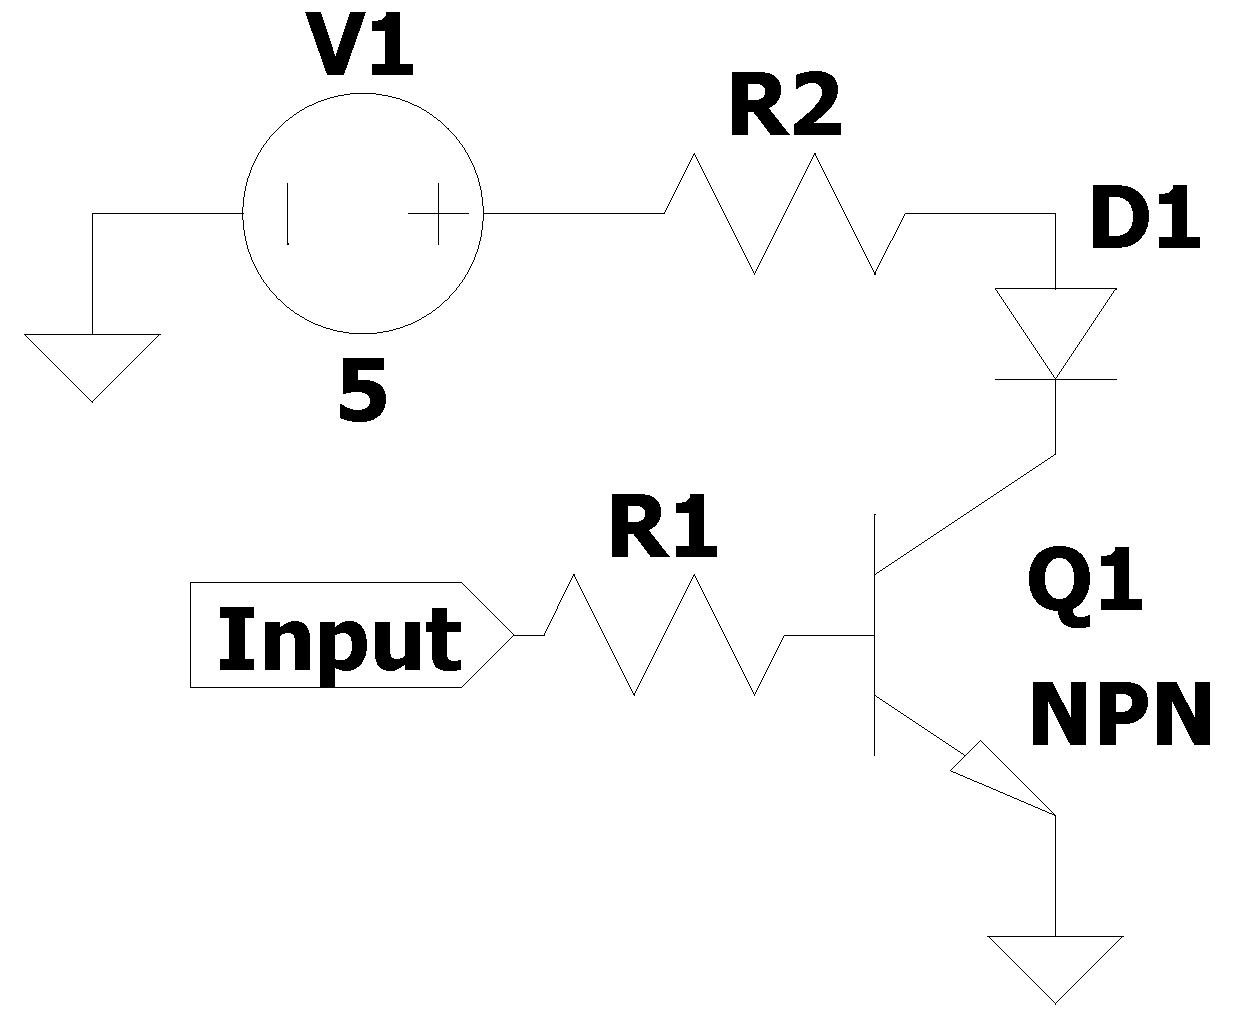
\includegraphics[width=0.5\textwidth]{figures/hardware_design/laser_transistor_schematic.pdf}
  \caption{Switching transistor circuit.}
  \label{fig:transistor_schematic}
\end{figure}

The stepper motors drivers were connected to the Nvidia Jetson Nano \gls{gpio} according to the diagram in \autoref{fig:stepper_driver_pins}.
\begin{figure}[h]
  \centering
  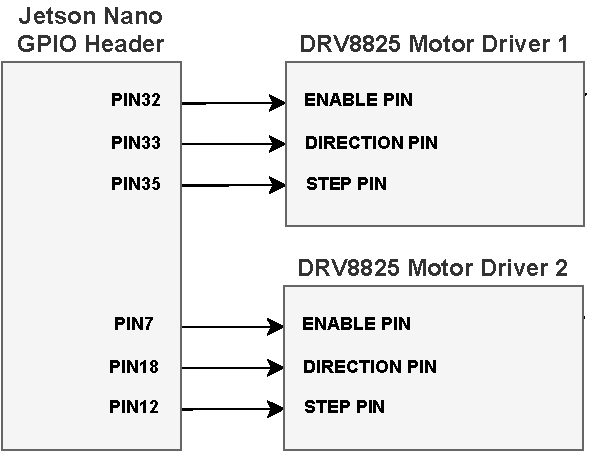
\includegraphics[width=0.6\textwidth]{figures/stepper_driver_pins.pdf}
  \caption{Stepper motor driver connections.}
  \label{fig:stepper_driver_pins}
\end{figure}
The motors are enabled by setting the \texttt{ENABLE PIN} to a logical high. The direction of rotation is determined by the logic level of the \texttt{DIRECTION PIN}. The stepper motors are driven by pulsing the \texttt{STEP PIN} at the desired frequency for the desired number of steps.

\newpage
\subsection{Record 4. Hardware acceptance test procedure}

\newpage
\subsection{Record 5. User guide}


%% --------------------------------------------------------------------

\newpage
\section{SOFTWARE part of the project}

\subsection{Record 6. Software process flow diagrams}
\begin{figure}[h]
  \centering
  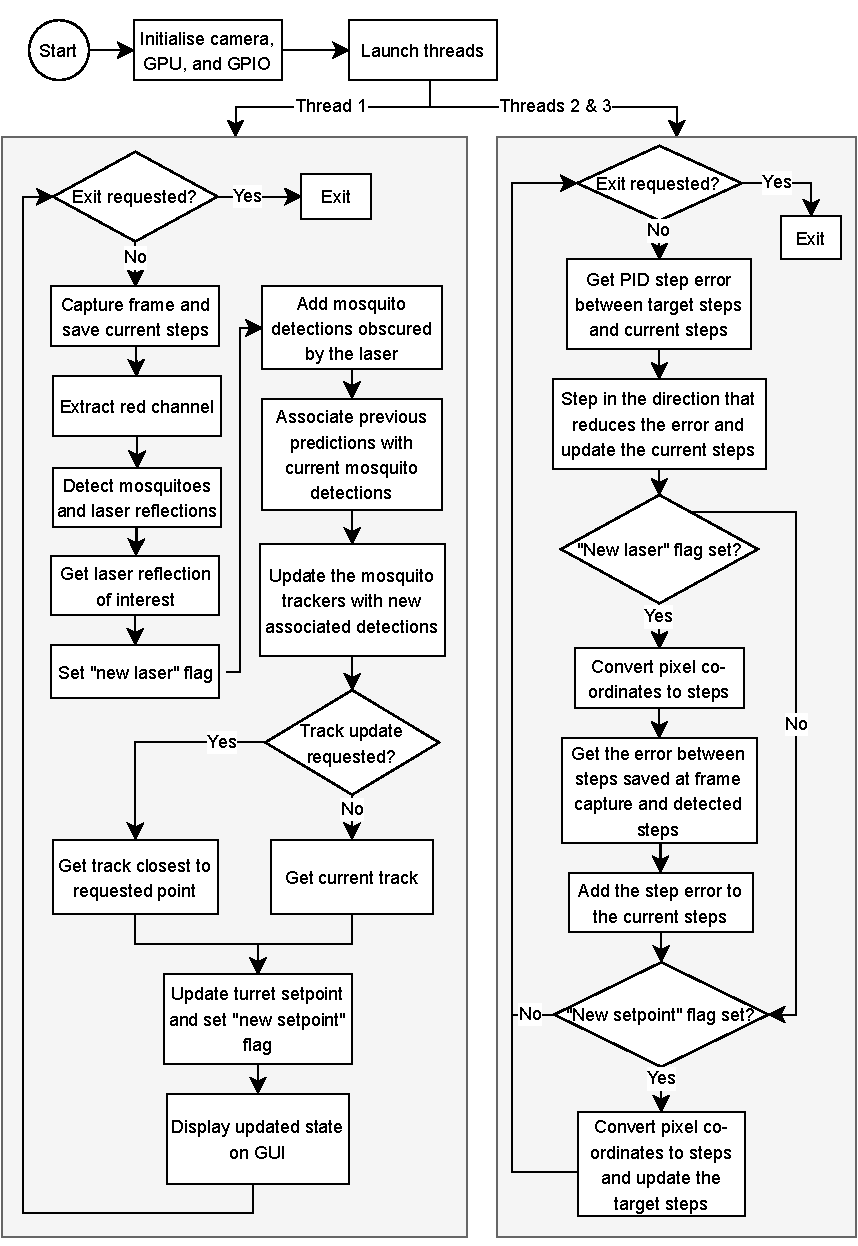
\includegraphics[width=0.95\textwidth]{figures/software_flow_diagram.pdf}
  \caption{Software flow diagram.}
\end{figure}

\newpage
\subsection{Record 7. Explanation of software modules}

\newpage
\subsection{Record 8. Complete source code}
Complete code has been submitted separately on the AMS.

\newpage
\subsection{Record 9. Software acceptance test procedure}

\newpage
\subsection{Record 10. Software user guide}


%% --------------------------------------------------------------------

\section{EXPERIMENTAL DATA}

\subsection{Record 11. Experimental data}


%% End of File.


